% !TEX program = pdflatex
% Compile TWICE: pdflatex main.tex && pdflatex main.tex
\documentclass[aspectratio=169,10pt]{beamer}

% ============================================================
%                    PACKAGES
% ============================================================
\usepackage[T1]{fontenc}
\usepackage{lmodern}
\usepackage{microtype}
\usepackage{tfrupee}            % provides \rupee
\usepackage{newunicodechar}
\newunicodechar{₹}{\rupee}

\usepackage{tikz}
\usetikzlibrary{positioning, calc}
\usepackage{booktabs}
\usepackage{array}
\usepackage{colortbl}
\usepackage{ragged2e}
\usepackage{amsmath}

% ============================================================
%               ROSE PINE PALETTE
% ============================================================
\definecolor{rpBase}{HTML}{FAF4ED}      % Main light background
\definecolor{rpSurface}{HTML}{FFFAF3}   % Slightly lighter surface
\definecolor{rpOverlay}{HTML}{F2E9E1}   % Overlay / UI background
\definecolor{rpMuted}{HTML}{9893A5}     % Muted text
\definecolor{rpSubtle}{HTML}{797593}    % Subtle text
\definecolor{rpText}{HTML}{575279}      % Main text (dark)
\definecolor{rpLove}{HTML}{B4637A}      % Love (red/pink accent)
\definecolor{rpGold}{HTML}{EA9D34}      % Gold (yellow/orange accent)
\definecolor{rpRose}{HTML}{D7827E}      % Rose (pink accent)
\definecolor{rpPine}{HTML}{286983}      % Pine (dark blue/green accent)
\definecolor{rpFoam}{HTML}{56949F}      % Foam (light blue/cyan accent)
\definecolor{rpIris}{HTML}{907AA9}      % Iris (purple accent)
\definecolor{rpHlMed}{HTML}{DFDAD9}     % Highlight Medium (for table rows)

% ============================================================
%               BEAMER THEME SETUP
% ============================================================
\setbeamertemplate{navigation symbols}{}
\setbeamercolor{background canvas}{bg=rpBase}
\setbeamercolor{normal text}{fg=rpText, bg=rpBase}
\setbeamercolor{structure}{fg=rpIris}
\setbeamercolor{frametitle}{fg=rpRose, bg=rpBase}
\setbeamercolor{title}{fg=rpIris}
\setbeamercolor{subtitle}{fg=rpRose}
\setbeamercolor{author}{fg=rpText}
\setbeamercolor{institute}{fg=rpSubtle}
\setbeamercolor{date}{fg=rpSubtle}
\setbeamercolor{itemize item}{fg=rpGold}
\setbeamercolor{itemize subitem}{fg=rpFoam}
\setbeamercolor{itemize subsubitem}{fg=rpLove}
\setbeamercolor{enumerate item}{fg=rpGold}
\setbeamercolor{block title}{fg=rpBase, bg=rpIris}
\setbeamercolor{block body}{fg=rpText, bg=rpSurface}
\setbeamercolor{block title alerted}{fg=rpBase, bg=rpLove}
\setbeamercolor{block body alerted}{fg=rpText, bg=rpSurface}
\setbeamercolor{block title example}{fg=rpBase, bg=rpPine}
\setbeamercolor{block body example}{fg=rpText, bg=rpSurface}
\setbeamercolor{section in toc}{fg=rpRose}

\setbeamerfont{frametitle}{size=\Large, series=\bfseries}
\setbeamerfont{title}{size=\Huge, series=\bfseries}
\setbeamerfont{subtitle}{size=\large, series=\itshape}

\setbeamertemplate{itemize item}{\textcolor{rpGold}{\small$\blacktriangleright$}}
\setbeamertemplate{itemize subitem}{\textcolor{rpFoam}{\scriptsize$\bullet$}}
\setbeamertemplate{itemize subsubitem}{\textcolor{rpLove}{\tiny$\circ$}}

\setbeamertemplate{frametitle}{
	\nointerlineskip
	\vskip8pt
	\hspace{0.35cm}\usebeamerfont{frametitle}\usebeamercolor[fg]{frametitle}\insertframetitle
	\vskip3pt
	\hspace{0.35cm}\textcolor{rpGold}{\rule{3.5cm}{0.9pt}}
	\vskip4pt
}

% ---- Footline: uses \hfil to absorb slack, so no overfull ----
\setbeamertemplate{footline}{
	\leavevmode
	\hbox to \paperwidth{%
		\hspace{0.35cm}%
		\begin{beamercolorbox}[wd=.31\paperwidth,ht=2.5ex,dp=1ex]{}
			\usebeamerfont{author in head/foot}\textcolor{rpMuted}{\small SEBI Act, 1992}%
		\end{beamercolorbox}%
		\begin{beamercolorbox}[wd=.32\paperwidth,ht=2.5ex,dp=1ex,center]{}
			\textcolor{rpMuted}{\small\insertshorttitle}%
		\end{beamercolorbox}%
		\begin{beamercolorbox}[wd=.31\paperwidth,ht=2.5ex,dp=1ex,right]{}
			\textcolor{rpMuted}{\small\insertframenumber\,/\,\inserttotalframenumber}%
		\end{beamercolorbox}%
		\hspace{0.35cm}%
		\hfil
	}%
	\vskip2pt
}

% ============================================================
%              SECTION DIVIDER MACRO
% ============================================================
\newcommand{\sectionslide}[2]{%
	\begin{frame}[plain]
		\begin{tikzpicture}[remember picture, overlay]
			\fill[rpBase] (current page.south west) rectangle (current page.north east);
			\fill[rpOverlay] ([xshift=-1.1cm]current page.north east)
			-- (current page.north east) -- (current page.south east)
			-- ([xshift=-1.1cm]current page.south east) -- cycle;
			\node[anchor=west, text=rpMuted, font=\fontsize{58}{58}\bfseries]
			at ([xshift=1.2cm]current page.west) {#1};
			\node[anchor=west, text=rpRose, font=\LARGE\bfseries]
			at ([xshift=5cm]current page.west) {#2};
			\draw[rpGold, line width=1.1pt]
			([xshift=5cm, yshift=-0.55cm]current page.west) -- ++(6.5cm,0);
		\end{tikzpicture}
	\end{frame}
}

% ============================================================
%              METADATA
% ============================================================
\title[SEBI Act, 1992]{The Securities and Exchange Board of India Act, 1992}
\subtitle{A Legislative and Architectural Overview}
\author{Neha Kumari \and Nitu Kumari \and Pallavi Singh}
\institute{Department of Commerce and Business Studies \\ \vspace{2pt} \small Guide: Mrs.\ Renu Rai}
\date{\today}

% ============================================================
\begin{document}
	
	% ------------------------------------------------------------
	%                    TITLE SLIDE
	% ------------------------------------------------------------
	% ------------------------------------------------------------
	%                    TITLE SLIDE (FIXED)
	% ------------------------------------------------------------
	\begin{frame}[plain]
		\begin{tikzpicture}[remember picture, overlay]
			% Background
			\fill[rpBase] (current page.south west) rectangle (current page.north east);
			
			% Bottom dark bar
			\fill[rpOverlay]
			([yshift=3.2cm]current page.south west)
			rectangle ([yshift=0.6cm]current page.south east);
			
			% Golden accent bar
			\fill[rpGold] ([yshift=3.3cm, xshift=0.6cm]current page.south west)
			rectangle ([yshift=3.2cm, xshift=5.5cm]current page.south west);
			
			% Top header rule
			\draw[rpIris, line width=1.4pt]
			([xshift=0.8cm, yshift=-0.7cm]current page.north west)
			-- ([xshift=6.5cm, yshift=-0.7cm]current page.north west);
			
			% Department Name
			\node[anchor=west, text=rpRose, font=\Large\bfseries]
			at ([xshift=0.8cm, yshift=-0.35cm]current page.north west)
			{Department of Commerce and Business Studies};
			
			% Academic Series Subtitle
			\node[anchor=west, text=rpMuted, font=\small\itshape]
			at ([xshift=0.8cm, yshift=-1.15cm]current page.north west)
			{Academic Presentation };
			
			% Main Title (FIXED: smaller font, wider width, pushed down)
			\node[anchor=west, text=rpText, font=\fontsize{26}{30}\bfseries, text width=14.5cm]
			at ([xshift=0.8cm, yshift=-2.9cm]current page.north west)
			{The Securities and Exchange Board of India Act, 1992};
			
			% Golden divider rule below title
			\draw[rpGold, line width=0.9pt]
			([xshift=0.8cm, yshift=-5.1cm]current page.north west) -- ++(4.5cm,0);
			
			% Legislative Subtitle
			\node[anchor=west, text=rpIris, font=\large\itshape]
			at ([xshift=0.8cm, yshift=-5.55cm]current page.north west)
			{A Legislative and Architectural Overview};
			
			% Bottom: Submitted by
			\node[anchor=west, text=rpText, font=\normalsize\bfseries]
			at ([xshift=0.8cm, yshift=1.7cm]current page.south west)
			{Submitted by};
			
			\node[anchor=west, text=rpFoam, font=\normalsize]
			at ([xshift=3.4cm, yshift=1.7cm]current page.south west)
			{Neha Kumari \quad\textbullet\quad Nitu Kumari \quad\textbullet\quad Pallavi Singh};
			
			% Bottom: Submitted to
			\node[anchor=west, text=rpText, font=\normalsize\bfseries]
			at ([xshift=0.8cm, yshift=0.9cm]current page.south west)
			{Submitted to};
			
			\node[anchor=west, text=rpRose, font=\normalsize]
			at ([xshift=3.4cm, yshift=0.9cm]current page.south west)
			{Mrs.\ Renu Rai};
		\end{tikzpicture}
	\end{frame}
	
	% ------------------------------------------------------------
	%                 TABLE OF CONTENTS
	% ------------------------------------------------------------
	% ------------------------------------------------------------
	%                 TABLE OF CONTENTS (FIXED)
	% ------------------------------------------------------------
	\begin{frame}{Table of Contents}
		\vspace{-0.2cm}
		\begin{columns}[T, onlytextwidth]
			\begin{column}{0.48\textwidth}
				\textcolor{rpIris}{\textbf{\footnotesize PART I --- FOUNDATIONS}}\\[2pt]
				\textcolor{rpText}{\footnotesize 1.\ Structure of the SEBI Act, 1992}\\[1pt]
				\textcolor{rpText}{\footnotesize 2.\ Legislative Overview}\\[1pt]
				\textcolor{rpText}{\footnotesize 3.\ An Architectural Glance}\\[1pt]
				\textcolor{rpText}{\footnotesize 4.\ Preliminary \& Board Setup}\\[4pt]
				
				\textcolor{rpIris}{\textbf{\footnotesize PART II --- POWERS \& INTERMEDIARIES}}\\[2pt]
				\textcolor{rpText}{\footnotesize 5.\ Powers \& Functions}\\[1pt]
				\textcolor{rpText}{\footnotesize 6.\ Registration \& Prohibitions}\\[4pt]
				
				\textcolor{rpIris}{\textbf{\footnotesize PART III --- ENFORCEMENT}}\\[2pt]
				\textcolor{rpText}{\footnotesize 7.\ Penalties \& Adjudication}\\[1pt]
				\textcolor{rpText}{\footnotesize 8.\ Securities Appellate Tribunal}\\[1pt]
				\textcolor{rpText}{\footnotesize 9.\ Penal Framework Comparison}\\[1pt]
				\textcolor{rpText}{\footnotesize 10.\ SEBI Act Chapter Breakdown}
			\end{column}
			\begin{column}{0.48\textwidth}
				\textcolor{rpIris}{\textbf{\footnotesize PART IV --- OVERSIGHT \& CASE LAW}}\\[2pt]
				\textcolor{rpText}{\footnotesize 11.\ Finance, Audit \& Government Oversight}\\[1pt]
				\textcolor{rpText}{\footnotesize 12.\ Case Study}\\[4pt]
				
				\textcolor{rpIris}{\textbf{\footnotesize PART V --- CLOSING}}\\[2pt]
				\textcolor{rpText}{\footnotesize 13.\ Conclusion}\\[1pt]
				\textcolor{rpText}{\footnotesize 14.\ References}\\[1pt]
				\textcolor{rpText}{\footnotesize 15.\ Thank You \& Query}\\[6pt]
				
				\begin{beamercolorbox}[rounded=true, sep=5pt, wd=\linewidth]{block body}
					\scriptsize \textcolor{rpRose}{\textbf{Aim:}} A concise structural reading of the SEBI Act --- from its statutory architecture to its enforcement machinery --- grounded in academic literature.
				\end{beamercolorbox}
			\end{column}
		\end{columns}
	\end{frame}
	
	% ============================================================
	\sectionslide{I}{Foundations of the Act}
	
	% ------------------------------------------------------------
	\begin{frame}{Structure of the SEBI Act, 1992}
		\begin{columns}[T, onlytextwidth]
			\begin{column}{0.58\textwidth}
				\vspace{0.2cm}
				{\large A detailed overview of the legislative framework establishing the Securities and Exchange Board of India, and defining its statutory mandate.}\\[10pt]
				\textcolor{rpMuted}{\rule{5cm}{0.6pt}}\\[10pt]
				\begin{itemize}
					\item Enacted by the Parliament of India in \textcolor{rpGold}{1992}.
					\item Establishes an \textcolor{rpIris}{autonomous statutory body}.
					\item Designed to balance \textcolor{rpRose}{market regulation} with \textcolor{rpFoam}{investor protection}.
					\item Structured across \textcolor{rpLove}{10 Chapters} and Sections 1 to 35.
				\end{itemize}
			\end{column}
			\begin{column}{0.38\textwidth}
				\vspace{0.4cm}
				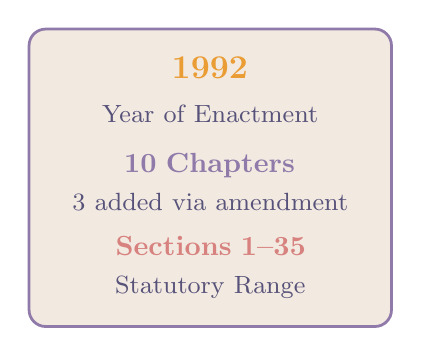
\begin{tikzpicture}
					\node[draw=rpIris, fill=rpOverlay, rounded corners=6pt,
					line width=1pt, inner sep=10pt, text width=3.9cm, align=center]
					{\textcolor{rpGold}{\textbf{\large 1992}}\\[4pt]
						\textcolor{rpText}{\small Year of Enactment}\\[6pt]
						\textcolor{rpIris}{\textbf{10 Chapters}}\\[2pt]
						\textcolor{rpText}{\small 3 added via amendment}\\[4pt]
						\textcolor{rpRose}{\textbf{Sections 1--35}}\\[2pt]
						\textcolor{rpText}{\small Statutory Range}};
				\end{tikzpicture}
			\end{column}
		\end{columns}
	\end{frame}
	
	% ------------------------------------------------------------
	% ------------------------------------------------------------
	\begin{frame}{Legislative Overview}
		\begin{columns}[T, onlytextwidth]
			\begin{column}{0.55\textwidth}
				\begin{block}{Statutory Framework}
					The \textbf{SEBI Act, 1992} was enacted to establish an autonomous statutory body for regulating India's securities market.
				\end{block}
				\vspace{4pt}
				\begin{itemize}
					\item Balances \textcolor{rpRose}{market regulation} with \textcolor{rpFoam}{investor protection}.
					\item Structured across \textcolor{rpGold}{10 Chapters} --- including \textcolor{rpIris}{VA, VIA, and VIB} added via amendments.
					\item Sections \textbf{1 to 35} define scope, powers, penalties, and appeals.
				\end{itemize}
			\end{column}
			\begin{column}{0.42\textwidth}
				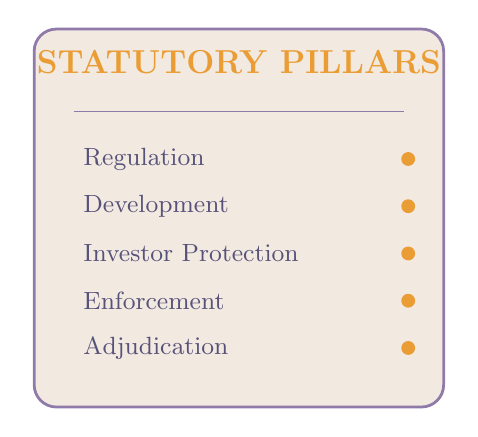
\begin{tikzpicture}
					% Outer box with balanced padding
					\draw[draw=rpIris, line width=1pt, fill=rpOverlay, rounded corners=8pt]
					(0,0) rectangle (5.2,4.8);
					
					% Title anchored to top to prevent overflow
					\node[anchor=north, text=rpGold, font=\large\bfseries] 
					at (2.6, 4.65) {STATUTORY PILLARS};
					
					% Divider
					\draw[rpIris, line width=0.4pt] (0.5,3.75) -- (4.7,3.75);
					
					% List items with balanced spacing
					\node[anchor=west, text=rpText] at (0.5,3.15) {\small Regulation};
					\node[anchor=west, text=rpText] at (0.5,2.55) {\small Development};
					\node[anchor=west, text=rpText] at (0.5,1.95) {\small Investor Protection};
					\node[anchor=west, text=rpText] at (0.5,1.35) {\small Enforcement};
					\node[anchor=west, text=rpText] at (0.5,0.75) {\small Adjudication};
					
					% Bullet points aligned to the right
					\foreach \y in {3.15,2.55,1.95,1.35,0.75}{
						\fill[rpGold] (4.75,\y) circle (2.5pt);
					}
				\end{tikzpicture}
			\end{column}
		\end{columns}
	\end{frame}
	
	% ------------------------------------------------------------
	% ------------------------------------------------------------
	\begin{frame}{An Architectural Glance}
		\vspace{-0.5cm}
		\centering
		\footnotesize
		\renewcommand{\arraystretch}{1.25}
		\arrayrulecolor{rpHlMed}
		\begin{tabular}{@{}>{\columncolor{rpOverlay}}p{2.2cm} p{2.3cm} p{7.8cm}@{}}
			\toprule
			\rowcolor{rpSurface}
			\textcolor{rpIris}{\textbf{Chapters}} & \textcolor{rpIris}{\textbf{Sections}} & \textcolor{rpIris}{\textbf{Subject Matter / Scope}}\\
			\midrule
			\rowcolor{rpOverlay} Chapter I        & Sec 1--2       & Preliminary: Short title, commencement, extent \& definitions \\
			\rowcolor{rpSurface} Chapter II       & Sec 3--9       & Establishment, incorporation \& management of the Board \\
			\rowcolor{rpOverlay} Chapter III      & Sec 10         & Transfer of assets, liabilities \& staff from predecessor board \\
			\rowcolor{rpSurface} Chapter IV       & Sec 11--11D    & Powers and statutory functions of SEBI \\
			\rowcolor{rpOverlay} Chapters V \& VA & Sec 12 \& 12A  & Registration of intermediaries \& prohibition of manipulative trades \\
			\rowcolor{rpSurface} Chapters VI--VII & Sec 13--35     & Finance, penalties, SAT establishment \& miscellaneous rules \\
			\bottomrule
		\end{tabular}
	\end{frame}
	
	% ------------------------------------------------------------
	% ------------------------------------------------------------
	\begin{frame}{Preliminary \& Board Setup}
		\vfill
		\begin{columns}[T]
			\begin{column}{0.31\textwidth}
				\begin{beamercolorbox}[rounded=true, sep=8pt]{block title}
					\centering\textbf{Preliminary}
				\end{beamercolorbox}
				\vspace{-2pt}
				\begin{beamercolorbox}[rounded=true, sep=10pt]{block body}
					\footnotesize \textbf{Sections 1--2:} Extends to whole of India. Defines key market concepts --- board, securities, market intermediaries, and regulatory authority.
				\end{beamercolorbox}
			\end{column}
			\begin{column}{0.31\textwidth}
				\begin{beamercolorbox}[rounded=true, sep=8pt]{block title}
					\centering\textbf{Establishment}
				\end{beamercolorbox}
				\vspace{-2pt}
				\begin{beamercolorbox}[rounded=true, sep=10pt]{block body}
					\footnotesize \textbf{Sections 3--9:} Establishes SEBI as a \textit{body corporate} with perpetual succession. Outlines board constitution, Chairman appointment, and meeting rules.
				\end{beamercolorbox}
			\end{column}
			\begin{column}{0.31\textwidth}
				\begin{beamercolorbox}[rounded=true, sep=8pt]{block title}
					\centering\textbf{Asset Transfer}
				\end{beamercolorbox}
				\vspace{-2pt}
				\begin{beamercolorbox}[rounded=true, sep=10pt]{block body}
					\footnotesize \textbf{Section 10:} Governs seamless transfer of assets, liabilities, contracts, and existing employees from the pre-statutory Board to SEBI.
				\end{beamercolorbox}
			\end{column}
		\end{columns}
		\vfill
	\end{frame}
	
	% ============================================================
	\sectionslide{II}{Powers, Functions \& Intermediaries}
	
	% ------------------------------------------------------------
	\begin{frame}{Powers \& Functions --- Core Mandate}
		\begin{columns}[T, onlytextwidth]
			\begin{column}{0.48\textwidth}
				\begin{block}{Core Regulatory Duty \textnormal{\small (Sec 11)}}
					\small Obligation to protect investor interests, promote capital market development, and regulate securities trading across India.
				\end{block}
				\begin{block}{Inspection \& Investigation \textnormal{\small (Sec 11C)}}
					\small Authority to conduct investigations into market abuses, call for information, and inspect books of registered intermediaries.
				\end{block}
			\end{column}
			\begin{column}{0.48\textwidth}
				\begin{block}{Directive Powers \textnormal{\small (Sec 11D)}}
					\small Power to issue \textit{Cease and Desist} orders against persons or entities indulging in fraudulent or unfair market activities.
				\end{block}
				\begin{block}{Market Intermediary Oversight}
					\small Power to mandate rules, audit stock exchanges and self-regulatory organisations, and supervise market participants.
				\end{block}
			\end{column}
		\end{columns}
	\end{frame}
	
	% ------------------------------------------------------------
	\begin{frame}{Registration \& Prohibitions}
		\begin{columns}[T, onlytextwidth]
			\begin{column}{0.48\textwidth}
				\begin{beamercolorbox}[rounded=true, sep=4pt]{block title}
					\centering\textbf{Chapter V --- Section 12}\\[2pt]
					\textcolor{rpBase}{\small Intermediary Registration}
				\end{beamercolorbox}
				\vspace{-4pt}
				\begin{beamercolorbox}[rounded=true, sep=5pt]{block body}
					\small Mandates compulsory \textit{Registration Certificates} for key market participants:
					\begin{itemize}\small
						\item Sub-Brokers \& Merchant Bankers
						\item Underwriters \& Portfolio Managers
						\item Investment Advisors
						\item Depository Participants \& Registrars
					\end{itemize}
				\end{beamercolorbox}
			\end{column}
			\begin{column}{0.48\textwidth}
				\begin{beamercolorbox}[rounded=true, sep=4pt]{block title alerted}
					\centering\textbf{Chapter V --- Section 12A}\\[2pt]
					\textcolor{rpBase}{\small Prohibited Activities}
				\end{beamercolorbox}
				\vspace{-4pt}
				\begin{beamercolorbox}[rounded=true, sep=5pt]{block body}
					\small Strictly prohibits illegal practices in securities transactions:
					\begin{itemize}\small
						\item Manipulative, deceptive devices or fraud
						\item Insider trading on non-public information
						\item Substantial acquisition without mandated disclosures
						\item Market manipulation \& price rigging
					\end{itemize}
				\end{beamercolorbox}
			\end{column}
		\end{columns}
	\end{frame}
	
	% ============================================================
	\sectionslide{III}{Enforcement \& Adjudication}
	
	% ------------------------------------------------------------
	\begin{frame}{Penalties \& Adjudication}
		\begin{columns}[T, onlytextwidth]
			\begin{column}{0.55\textwidth}
				\begin{block}{Monetary Sanctions \textnormal{\small (Sec 15A--15HB)}}
					\small Specific penalties for failure to furnish information, non-disclosure of insider holdings, insider trading, and broker defaults.
				\end{block}
				\begin{block}{Adjudicating Officers \textnormal{\small (Sec 15I)}}
					\small SEBI appoints officers to hold inquiry and impose statutory monetary fines based on the nature and extent of default.
				\end{block}
				\begin{block}{Settlement Proceedings \textnormal{\small (Sec 15JB)}}
					\small Provision for settlement of administrative enforcement proceedings, with or without admission of guilt.
				\end{block}
			\end{column}
			\begin{column}{0.42\textwidth}
				\vspace{0.3cm}
				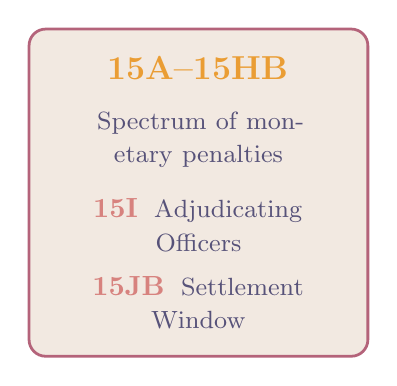
\begin{tikzpicture}
					\node[draw=rpLove, fill=rpOverlay, rounded corners=6pt,
					line width=1pt, inner sep=10pt, text width=3.6cm, align=center]
					{\textcolor{rpGold}{\textbf{\large 15A--15HB}}\\[6pt]
						\textcolor{rpText}{\small Spectrum of monetary penalties}\\[8pt]
						\textcolor{rpRose}{\textbf{15I}} \textcolor{rpText}{\small \;Adjudicating Officers}\\[4pt]
						\textcolor{rpRose}{\textbf{15JB}} \textcolor{rpText}{\small \;Settlement Window}};
				\end{tikzpicture}
			\end{column}
		\end{columns}
	\end{frame}
	
	% ------------------------------------------------------------
	\begin{frame}{Securities Appellate Tribunal}
		\vspace{0.1cm}
		\begin{center}
			\textcolor{rpIris}{\textbf{Chapter VIB (Sections 15K--15Z) --- Judicial Mechanism for Appeals}}
		\end{center}
		\vspace{0.3cm}
		\begin{columns}[T, onlytextwidth]
			\begin{column}{0.25\textwidth}
				\centering
				
\begin{tikzpicture}
					\node[draw=rpGold, fill=rpOverlay, circle, line width=1.2pt,
					minimum size=1.1cm, text=rpGold, font=\bfseries] {1};
				\end{tikzpicture}\\[4pt]
				\textcolor{rpRose}{\textbf{\small SEBI Order}}\\[2pt]
				\textcolor{rpText}{\scriptsize Adjudicating Officer or Board issues a regulatory order or penalty.}
			\end{column}
			\begin{column}{0.25\textwidth}
				\centering
				
\begin{tikzpicture}
					\node[draw=rpIris, fill=rpOverlay, circle, line width=1.2pt,
					minimum size=1.1cm, text=rpIris, font=\bfseries] {2};
				\end{tikzpicture}\\[4pt]
				\textcolor{rpRose}{\textbf{\small Appeal to SAT}}\\[2pt]
				\textcolor{rpText}{\scriptsize File appeal under Sec 15T within 45 days of receiving the order.}
			\end{column}
			\begin{column}{0.25\textwidth}
				\centering
				
\begin{tikzpicture}
					\node[draw=rpFoam, fill=rpOverlay, circle, line width=1.2pt,
					minimum size=1.1cm, text=rpFoam, font=\bfseries] {3};
				\end{tikzpicture}\\[4pt]
				\textcolor{rpRose}{\textbf{\small SAT Proceeding}}\\[2pt]
				\textcolor{rpText}{\scriptsize SAT exercises civil court powers (Sec 15U) to hear \& pass judgment.}
			\end{column}
			\begin{column}{0.25\textwidth}
				\centering
				
\begin{tikzpicture}
					\node[draw=rpLove, fill=rpOverlay, circle, line width=1.2pt,
					minimum size=1.1cm, text=rpLove, font=\bfseries] {4};
				\end{tikzpicture}\\[4pt]
				\textcolor{rpRose}{\textbf{\small Supreme Court}}\\[2pt]
				\textcolor{rpText}{\scriptsize Further appeal on law questions within 60 days (Sec 15Z).}
			\end{column}
		\end{columns}
	\end{frame}
	
	% ------------------------------------------------------------
	\begin{frame}{Penal Framework Comparison}
		\vspace{-0.1cm}
		\centering
		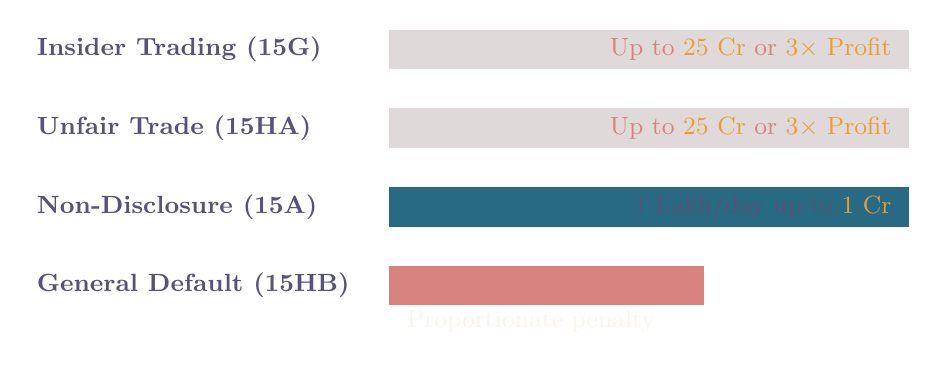
\begin{tikzpicture}
			\node[anchor=west, text=rpText, font=\small\bfseries] at (0,3.1) {Insider Trading (15G)};
			\fill[rpHlMed] (4.6,3.35) rectangle (11.2,2.85);
			\node[anchor=east, text=rpRose, font=\small] at (11.1,3.1)
			{Up to \textcolor{rpGold}{\rupee 25 Cr} or \textcolor{rpGold}{3$\times$ Profit}};
			
			\node[anchor=west, text=rpText, font=\small\bfseries] at (0,2.1) {Unfair Trade (15HA)};
			\fill[rpHlMed] (4.6,2.35) rectangle (11.2,1.85);
			\node[anchor=east, text=rpRose, font=\small] at (11.1,2.1)
			{Up to \textcolor{rpGold}{\rupee 25 Cr} or \textcolor{rpGold}{3$\times$ Profit}};
			
			\node[anchor=west, text=rpText, font=\small\bfseries] at (0,1.1) {Non-Disclosure (15A)};
			\fill[rpPine] (4.6,1.35) rectangle (11.2,0.85);
			\node[anchor=east, text=rpText, font=\small] at (11.1,1.1)
			{\rupee 1 Lakh/day up to \textcolor{rpGold}{\rupee 1 Cr}};
			
			\node[anchor=west, text=rpText, font=\small\bfseries] at (0,0.1) {General Default (15HB)};
			\fill[rpRose] (4.6,0.35) rectangle (8.6,-0.15);
			\node[anchor=west, text=rpBase, font=\small] at (4.7,-0.35) {Proportionate penalty};
		\end{tikzpicture}
		
		\vspace{0.25cm}
		\textcolor{rpMuted}{\small Comparison of statutory maximum penalties under Chapter VIA of the SEBI Act, 1992 --- reflecting the severe treatment of market-integrity breaches.}
	\end{frame}
	
	% ------------------------------------------------------------
	\begin{frame}{SEBI Act --- Chapter Breakdown}
		\vspace{-0.1cm}
		\centering
		\renewcommand{\arraystretch}{1.55}
		\arrayrulecolor{rpHlMed}
		\begin{tabular}{@{}>{\columncolor{rpOverlay}}p{2.3cm} p{2.3cm} p{5.3cm} p{3.4cm}@{}}
			\toprule
			\rowcolor{rpSurface}
			\textcolor{rpIris}{\textbf{Chapters}} & \textcolor{rpIris}{\textbf{Sections}} & \textcolor{rpIris}{\textbf{Key Provisions}} & \textcolor{rpIris}{\textbf{Primary Focus}}\\
			\midrule
			\rowcolor{rpOverlay} I--III      & 1--10     & Establishment, definitions \& Board setup    & Institutional Governance\\
			\rowcolor{rpSurface} IV--V       & 11--12    & Powers, registration \& inspections          & Market Intermediary Control\\
			\rowcolor{rpOverlay} VA          & 12A       & Fraud, Insider Trading \& Takeovers          & Market Integrity \& Ethics\\
			\rowcolor{rpSurface} VIA--VIB    & 15A--15Z  & Adjudication, Penalties \& SAT Appeals       & Enforcement \& Appellate Remedies\\
			\rowcolor{rpOverlay} VI--VII     & 13--35    & Finance, Audit, Rules \& CG Powers           & Financial \& Policy Oversight\\
			\bottomrule
		\end{tabular}
	\end{frame}
	
	% ============================================================
	\sectionslide{IV}{Oversight \& Case Law}
	
	% ------------------------------------------------------------
	\begin{frame}{Finance, Audit \& Government Oversight}
		\begin{columns}[T, onlytextwidth]
			\begin{column}{0.48\textwidth}
				\begin{beamercolorbox}[rounded=true, sep=4pt]{block title}
					\centering\textbf{Chapter VI \; (Sec 13--15)}\\[2pt]
					\textcolor{rpBase}{\small Finance \& Audit}
				\end{beamercolorbox}
				\vspace{-4pt}
				\begin{beamercolorbox}[rounded=true, sep=5pt]{block body}
					\small
					\textbf{Grants \& Fund:} SEBI maintains a separate fund for fees, charges, and central grants received.\\[6pt]
					\textbf{Accounts \& Audit:} Accounts audited annually by the \textit{Comptroller and Auditor-General of India (CAG)}.
				\end{beamercolorbox}
			\end{column}
			\begin{column}{0.48\textwidth}
				\begin{beamercolorbox}[rounded=true, sep=4pt]{block title alerted}
					\centering\textbf{Chapter VII \; (Sec 16--35)}\\[2pt]
					\textcolor{rpBase}{\small Government Directives \& Rules}
				\end{beamercolorbox}
				\vspace{-4pt}
				\begin{beamercolorbox}[rounded=true, sep=5pt]{block body}
					\small
					\textbf{Central Powers:} Government power to issue binding policy directions (\textcolor{rpGold}{Sec 16}) and to supersede the Board in emergencies (\textcolor{rpGold}{Sec 17}).\\[6pt]
					Provides a constitutional safeguard over the regulator's autonomy.
				\end{beamercolorbox}
			\end{column}
		\end{columns}
	\end{frame}
	
	% ------------------------------------------------------------
	% ------------------------------------------------------------
	\begin{frame}{Case Study}
		\vfill
		\begin{columns}[T]
			\begin{column}{0.31\textwidth}
				\begin{beamercolorbox}[rounded=true, sep=8pt]{block title}
					\centering\textbf{Harshad Mehta Scam}\\[2pt]
					\textcolor{rpBase}{\small 1992}
				\end{beamercolorbox}
				\vspace{-2pt}
				\begin{beamercolorbox}[rounded=true, sep=10pt]{block body}
					\footnotesize A watershed securities fraud that catalysed a stronger, statutory role for SEBI in market regulation.
				\end{beamercolorbox}
			\end{column}
			\begin{column}{0.31\textwidth}
				\begin{beamercolorbox}[rounded=true, sep=8pt]{block title}
					\centering\textbf{Satyam Scandal}\\[2pt]
					\textcolor{rpBase}{\small 2009}
				\end{beamercolorbox}
				\vspace{-2pt}
				\begin{beamercolorbox}[rounded=true, sep=10pt]{block body}
					\footnotesize Triggered sweeping corporate governance reforms, sharpening disclosure norms and board accountability.
				\end{beamercolorbox}
			\end{column}
			\begin{column}{0.31\textwidth}
				\begin{beamercolorbox}[rounded=true, sep=8pt]{block title}
					\centering\textbf{Recent IPO Oversight}\\[2pt]
					\textcolor{rpBase}{\small Present Day}
				\end{beamercolorbox}
				\vspace{-2pt}
				\begin{beamercolorbox}[rounded=true, sep=10pt]{block body}
					\footnotesize Ensuring fair allotment, transparent disclosures, and orderly participation in primary markets.
				\end{beamercolorbox}
			\end{column}
		\end{columns}
		\vfill
	\end{frame}
	
	% ============================================================
	\sectionslide{V}{Conclusion \& References}
	
	% ------------------------------------------------------------
	\begin{frame}{Conclusion}
		\begin{columns}[T, onlytextwidth]
			\begin{column}{0.55\textwidth}
				\begin{itemize}
					\item Ensures \textcolor{rpGold}{market integrity} through a robust statutory framework.
					\item Builds \textcolor{rpFoam}{investor confidence} via transparent enforcement.
					\item Promotes \textcolor{rpRose}{financial inclusion} by widening safe market access.
					\item Aligns Indian markets with \textcolor{rpIris}{global regulatory standards}.
				\end{itemize}
			\end{column}
			\begin{column}{0.42\textwidth}
				\vspace{0.3cm}
				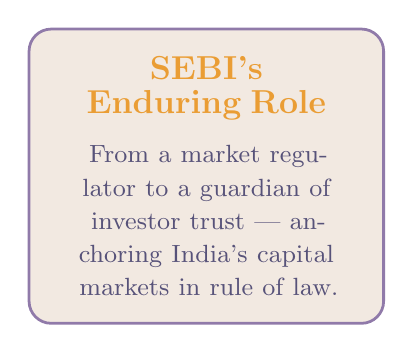
\begin{tikzpicture}
					\node[draw=rpIris, fill=rpOverlay, rounded corners=8pt,
					line width=1pt, inner sep=10pt, text width=3.8cm, align=center]
					{\textcolor{rpGold}{\textbf{\large SEBI's \\ Enduring Role}}\\[6pt]
						\textcolor{rpText}{\small From a market regulator to a guardian of investor trust --- anchoring India's capital markets in rule of law.}};
				\end{tikzpicture}
			\end{column}
		\end{columns}
	\end{frame}
	
	% ------------------------------------------------------------
	% References: \sloppy + \footnotesize eliminates overfull
	% ------------------------------------------------------------
	\begin{frame}{References}
		\sloppy
		\begin{columns}[T, onlytextwidth]
			\begin{column}{0.48\textwidth}
				\color{rpText}\footnotesize
				\textcolor{rpIris}{\textbf{Books}}\\[3pt]
				\textbullet\ Pathak, B.\,V.\ (2018). \textit{Indian Financial System: Markets, Institutions and Services} (5th ed.). Pearson Education.\\[3pt]
				\textbullet\ Das, S.\,C.\ (2025). \textit{The Financial System in India: Markets, Instruments, Institutions, Services and Regulations}. PHI Learning.\\[3pt]
				\textbullet\ Saha, S.\,S.\ (2021). \textit{Indian Financial System}. McGraw Hill.\\[6pt]
				\textcolor{rpIris}{\textbf{Newspapers}}\\[3pt]
				\textbullet\ The Economic Times\\[1pt]
				\textbullet\ The Financial Express\\[1pt]
				\textbullet\ Mint\\[1pt]
				\textbullet\ Business Line
			\end{column}
			\begin{column}{0.48\textwidth}
				\color{rpText}\footnotesize
				\textcolor{rpIris}{\textbf{Official Sources}}\\[3pt]
				\textbullet\ Securities and Exchange Board of India --- Official Website\\[3pt]
				\textbullet\ Department of Economic Affairs, Ministry of Finance\\[6pt]
				\textcolor{rpIris}{\textbf{Statute}}\\[3pt]
				\textbullet\ The Securities and Exchange Board of India Act, 1992 (Act No.\,15 of 1992), as amended.\\[8pt]
				\begin{beamercolorbox}[rounded=true, sep=5pt]{block body}
					\scriptsize \textcolor{rpMuted}{All quotations and statutory references are drawn from the official Act and standard academic texts.}
				\end{beamercolorbox}
			\end{column}
		\end{columns}
	\end{frame}
	
	% ------------------------------------------------------------
	\begin{frame}[plain]
		\begin{tikzpicture}[remember picture, overlay]
			\fill[rpBase] (current page.south west) rectangle (current page.north east);
			\fill[rpOverlay]
			([xshift=-4cm, yshift=-3cm]current page.north east)
			circle (5cm);
			\fill[rpOverlay]
			([xshift=4cm, yshift=3cm]current page.south west)
			circle (5cm);
			
			\node[text=rpText, font=\fontsize{46}{50}\bfseries]
			at ([yshift=0.9cm]current page.center) {THANK YOU};
			\draw[rpGold, line width=1.4pt]
			([yshift=0.15cm, xshift=-3cm]current page.center)
			-- ([yshift=0.15cm, xshift=3cm]current page.center);
			\node[text=rpRose, font=\large\itshape]
			at ([yshift=-0.7cm]current page.center) {Questions \& Discussion};
			\node[text=rpMuted, font=\small]
			at ([yshift=-1.6cm]current page.center)
			{Neha Kumari \;\textbullet\; Nitu Kumari \;\textbullet\; Pallavi Singh};
		\end{tikzpicture}
	\end{frame}
	
\end{document}